\documentclass[11pt]{article}
\usepackage{times}
\usepackage[margin=1in]{geometry}
\usepackage{amsmath}
\usepackage{amssymb}
\usepackage{amsthm}
\usepackage{graphicx}
\graphicspath{{../solutions/figures/}}
\usepackage{fancyhdr}
\usepackage{parskip}
\usepackage{sourcecodepro}
\usepackage{listings}
\usepackage{color}
\usepackage{hyperref}

% --- edit for submission ---
\newcommand{\StudentName}{Daniel (UNI: dad2232)}

% Header setup
\pagestyle{fancy}
\fancyhf{}
\rhead{Name: \StudentName}
\lhead{APMA 4302 - Methods}
\cfoot{\thepage}

\begin{document}
\lstset{basicstyle=\ttfamily}

\title{APMA 4302 Methods - Homework 3: Non-linear solver for reaction-diffusion equations}
\author{\StudentName \\[0.5em]\small Assignment: Marc Spiegelman}
\date{\today}
\maketitle

Here we will solve the nonlinear reaction-diffusion equation
\begin{displaymath}
  -\mathbf{\nabla}^2 u + \gamma u^p = f
\end{displaymath}
on the unit square with  non-homogeneous Dirichlet boundary conditions. Here $\gamma$ is a positive constant and $p>1$ is an integer. The right-hand side $f$ will be determined by the method of manufactured solutions, assuming the exact solution is given by
\begin{displaymath}
  u_{exact}(x,y) = A \exp\left(-\frac{(x-x_0)^2+(y-y_0)^2}{\sigma^2}\right),
\end{displaymath}
where $(x_0,y_0)$ is a point in the unit square and $\sigma$ is a positive constant controlling the width of the Gaussian of maximum amplitude $A$.

To help with this exercise, I have provided the code \texttt{poisson2d.c} in the \texttt{apma4302-methods} repository which solves the linear version of this problem (i.e. $\gamma=0$) as the discrete problem $A\mathbf{x}=\mathbf{b}$ as well as providing \texttt{VTK} output for visualizing in \href{https://www.paraview.org/}{ParaView}.

Do the following:
\begin{enumerate}
  \item (\textbf{5 pts}) Use finite differences to discretize the nonlinear PDE and write down the resulting nonlinear system of equations  in the form $F(\mathbf{u})=0$. Include auxiliary equations for non-homogeneous Dirichlet boundary conditions.
  \item (\textbf{5 pts}) Provide equations for elements of the  Jacobian matrix $J_{i,j}(\mathbf{u})=\frac{\partial F_i}{\partial u_j}$.
  \item (\textbf{20 pts}) Modify the code \texttt{reaction.c} in the \texttt{p4pdes} repository to solve the nonlinear problem using Newton's method with the \texttt{PETSc SNES} objects. Your code should have the following properties.
    \begin{enumerate}
      \item It should run with the interface
    \begin{verbatim}
    mpirun -n <num_procs> ./reaction2d  -rct_p <p>
            -rct_gamma <gamma> -rct_linear_f
    \end{verbatim}
        plus standard petsc command-line options.

        The option \texttt{-rct\_linear\_f} should be a boolean flag such that if true, sets the right-hand side to be
        \begin{displaymath}
          f(x,y) = - \mathbf{\nabla}^2 u_{exact}
        \end{displaymath}
        (i.e. the RHS for the linear problem) and if false, sets the right-hand side to be the full nonlinear RHS for the manufactured solution
        \begin{displaymath}
          f(x,y) = - \mathbf{\nabla}^2 u_{exact} + \gamma u_{exact}^p
        \end{displaymath}
        You can use the code in \texttt{poisson2d.c} to calculate $u_{exact}$ and its derivatives.
      \item Boundary conditions should be $u_{exact}$ on all boundaries, independent of the value of \texttt{-rct\_linear\_f}.
      \item It should include routines to compute both the nonlinear residual $F(\mathbf{u})$ and the Jacobian matrix $J(\mathbf{u})$.
      \item It should also be able to run with Finite difference jacobians using the options \texttt{-snes\_fd}, \texttt{-snes\_fd\_color}, \texttt{-snes\_mf} and \texttt{-snes\_mf\_operator} and should give the same results as the user-provided Jacobian. (you can use the option \texttt{-snes\_test\_jacobians} to check.
        \item It should output the solution in \texttt{VTK} format for visualization in \texttt{ParaView}.
      \end{enumerate}
    \item (\textbf{5 pts}) Run your code with $\gamma=0$ for a $65 \times 65$ grid and show that the linear and nonlinear solvers produce the same solution within error.  Find an appropriate set of linear solver options and stopping conditions so that the non-linear solver converges to a residual norm $\|F(\mathbf{u})\|_2 < 10^{-10}$ in one newton iteration. Report the number of linear iterations taken at each Newton step and the final \emph{relative error}  $\|\mathbf{u}-\mathbf{u}_{exact}\|_2/\|\mathbf{u}_{exact}\|_2$. (hint: some useful command line options include \texttt{-ksp\_monitor}, \texttt{-snes\_monitor}, \texttt{-ksp\_rtol} and \texttt{-ksp\_atol}). Feel free to experiment with different linear solvers and preconditioners (including sparse-direct solvers), but your code should run in parallel. Save your preferred options in a file \texttt{options\_file\_gamma0} and include it with your submission.
    \item (\textbf{2 pts}) Show that you get the same solution with the finite-difference Jacobian and report any differences in convergence behavior or final error. Include the command line options you used to run with the finite-difference Jacobian in a file \texttt{options\_file\_fd} and include it with your submission. Compare the run times for the user-provided Jacobian and the finite-difference Jacobian and report any differences. (hint: use \texttt{-log\_view} to get detailed timing information).
    \item (\textbf{5 pts}) Now set $\gamma=100$ and $p=3$ and run the nonlinear solver with the same stopping conditions as before. Report the number of Newton iterations taken, the number of linear iterations taken at each Newton step and the final \emph{relative error} $\|\mathbf{u}-\mathbf{u}_{exact}\|_2/\|\mathbf{u}_{exact}\|_2$. Plot the convergence history of the nonlinear residual norm $\|F(\mathbf{u})\|_2$.
    \item (\textbf{5 pts}) rerun the problem with \texttt{-rct\_linear\_f} and visualize the solution for $\gamma=100$ and $p=3$ in \texttt{ParaView} and include a screenshot of the solution in your submission. Describe how the nonlinearity has affected the solution compared to the linear case $\gamma=0$.
    \item (\textbf{10 pts}) \textbf{Performance and scaling} make a table (and/or plot) comparing
      \begin{itemize}
        \item run times (use \texttt{-log\_view})
        \item  number of Newton iterations
        \item relative norm of the error $\|\mathbf{u}-\mathbf{u}_{exact}\|_2/\|\mathbf{u}_{exact}\|_2$
      \end{itemize}
      for the non-linear problem for \texttt{-da\_refine} $2,3,4,5,6$ (i.e. grid sizes of $33\times 33$, to $513\times 513$) and 1,2 and 4 processors. I may actually provide a script for this part. Comment on the scaling of the code with respect to both problem size and number of processors.
  \end{enumerate}

% ---------------------------------------------------------------------------
% Written solutions: Problems 1 and 2
% ---------------------------------------------------------------------------
\section*{Written solutions}

\subsection*{Problem 1 --- Discrete system $F(\mathbf{u})=\mathbf{0}$}

\paragraph{What the question asks.}
Part~1 wants the PDE
\[
  -\nabla^2 u + \gamma\, u^{p} = f
\]
on $[0,1]\times[0,1]$ turned into a \emph{finite set} of nonlinear algebraic equations. Stack all unknown nodal values into a vector $\mathbf{u}$; each equation is one component of $F(\mathbf{u})$, and the boundary data appear as their own rows (``auxiliary'' equations), not by silently eliminating boundary unknowns.

\paragraph{Grid and notation.}
Place a uniform tensor-product grid with mesh spacing $h=1/N$ and nodes
\[
  (x_i,y_j) = (ih,jh),\qquad i,j \in \{0,1,\ldots,N\},
\]
so there are $(N{+}1)^2$ nodes. Let $u_{i,j}\approx u(x_i,y_j)$ and $f_{i,j}=f(x_i,y_j)$. Denote boundary values of the manufactured solution by
\[
  g_{i,j} := u_{\mathrm{exact}}(x_i,y_j).
\]

\paragraph{Five-point Laplacian.}
For an interior node ($1\le i\le N-1$, $1\le j\le N-1$), use the standard second-order centered stencil
\[
  (\nabla^2 u)_{i,j} \approx \frac{u_{i-1,j}+u_{i+1,j}+u_{i,j-1}+u_{i,j+1}-4u_{i,j}}{h^2}.
\]
Substituting into the PDE and moving everything to one side gives the \emph{interior} residual equations
\begin{equation}
\label{eq:Finterior}
  F_{i,j}(\mathbf{u})
  := -\frac{u_{i-1,j}+u_{i+1,j}+u_{i,j-1}+u_{i,j+1}-4u_{i,j}}{h^2}
     + \gamma\, u_{i,j}^{p} - f_{i,j}
  = 0.
\end{equation}

\paragraph{Non-homogeneous Dirichlet boundary conditions.}
On the boundary ($i\in\{0,N\}$ or $j\in\{0,N\}$), the physical boundary condition is $u=u_{\mathrm{exact}}$. In the algebraic system this is enforced by \emph{auxiliary equations} that involve only the boundary unknowns and the prescribed data:
\begin{equation}
\label{eq:Fbc}
  F_{i,j}(\mathbf{u}) := u_{i,j} - g_{i,j} = 0
  \qquad\text{for all boundary nodes } (i,j).
\end{equation}
Together, \eqref{eq:Finterior} on the interior and \eqref{eq:Fbc} on the boundary define $F_{i,j}$ at every node. After choosing a bijection from double indices $(i,j)$ to a single index $m\in\{1,\ldots,(N+1)^2\}$ (for example row-major order $m = i + j(N{+}1) + 1$), one obtains a vector-valued map $F:\mathbb{R}^{(N+1)^2}\to\mathbb{R}^{(N+1)^2}$ with components $F_m(\mathbf{u})=0$. This is the required form $F(\mathbf{u})=\mathbf{0}$.

\subsection*{Problem 2 --- Jacobian entries $J_{mn}=\partial F_m/\partial u_n$}

Let the unknowns be ordered consistently with the residual: $u_n$ denotes the value at the node corresponding to index $n$. The Jacobian $J(\mathbf{u})=F'(\mathbf{u})$ is sparse: each interior equation couples at most five unknowns (center and four neighbors), and each boundary equation couples only one.

\paragraph{Boundary rows.}
If equation $m$ is the boundary equation $u_{i,j}-g_{i,j}=0$ at node $(i,j)$, then
\[
  \frac{\partial F_m}{\partial u_n} =
  \begin{cases}
    1, & \text{if $n$ indexes the same node $(i,j)$,}\\
    0, & \text{otherwise.}
  \end{cases}
\]
Thus each boundary row of $J$ is a single~$1$ on the diagonal (in the natural ordering where equation and unknown refer to the same node).

\paragraph{Interior rows.}
If equation $m$ is the interior residual \eqref{eq:Finterior} at node $(i,j)$, denote partial differentiation with respect to the nodal value at $(r,s)$ by $\partial_{(r,s)}$. For any neighbor $(r,s)\in\{(i\pm1,j),(i,j\pm1)\}$,
\[
  \frac{\partial F_m}{\partial u_{r,s}}
  = -\frac{1}{h^2},
\]
for the center node,
\[
  \frac{\partial F_m}{\partial u_{i,j}}
  = \frac{4}{h^2} + \gamma\, p\, u_{i,j}^{\,p-1},
\]
and $\partial F_m/\partial u_{r,s}=0$ for all other $(r,s)$. In words: the Laplacian part contributes the usual five-point pattern scaled by $1/h^2$ (neighbor entries $-1/h^2$, center $+4/h^2$), and the reaction term adds a diagonal contribution $\gamma p u^{p-1}$ at that node.

\paragraph{Structure for Newton's method.}
With the ordering above, $J(\mathbf{u})$ has the sparsity of a five-point stencil on interior rows, plus pointwise modifications on the diagonal from $\gamma p u^{p-1}$, while boundary rows make the corresponding diagonal entries equal to~$1$ and zero out the rest of those rows. This matches what a hand-assembled SNES Jacobian should implement (up to equivalent orderings used in code).

\subsection*{Problem 3 --- Implementation (\texttt{reaction2d})}

The program \texttt{reaction2d} lives in \path{p4pdes/c/ch4/reaction2d.c} and is built with \texttt{make reaction2d}. Nonlinear solves use \texttt{PETSc} \texttt{SNES} on a 2D \texttt{DMDA} over $[0,1]\times[0,1]$.

\paragraph{(a) Command-line interface and choice of $f(x,y)$.}
The solver is invoked as
\begin{verbatim}
mpirun -n <num_procs> ./reaction2d -rct_p <p> -rct_gamma <gamma> [-rct_linear_f]
    [standard PETSc options ...]
\end{verbatim}
Options use the prefix \texttt{-rct\_} (\texttt{PetscOptionsBegin(...,"rct\_",...)}). Here \texttt{-rct\_p} sets the integer exponent~$p$ and \texttt{-rct\_gamma} sets~$\gamma$. The flag \texttt{-rct\_linear\_f} is a \texttt{PetscBool}: if \textbf{true} (flag present), the code uses the linear MMS forcing
\begin{displaymath}
  f(x,y) = -\nabla^2 u_{\mathrm{exact}}(x,y),
\end{displaymath}
implemented with the same \texttt{d2ufunction} as \texttt{poisson2d.c} (Laplacian of the Gaussian). If \textbf{false} (default), it uses the full nonlinear MMS forcing
\begin{displaymath}
  f(x,y) = -\nabla^2 u_{\mathrm{exact}}(x,y) + \gamma\, u_{\mathrm{exact}}(x,y)^{p}.
\end{displaymath}
The field $u_{\mathrm{exact}}$ is evaluated with \texttt{ufunction} from \texttt{poisson2d.c}. An additional flag \texttt{-rct\_zero\_initial} starts the iterate from $\mathbf{u}=\mathbf{0}$ (default is $u_{\mathrm{exact}}$, useful for MMS). Any additional \texttt{PETSc} options (e.g.\ \texttt{-da\_refine}, \texttt{-ksp\_*}, \texttt{-snes\_*}, \texttt{-pc\_*}) are passed through as usual.

\paragraph{(b) Boundary conditions.}
On all four sides of the square, Dirichlet data are $u = u_{\mathrm{exact}}$ regardless of \texttt{-rct\_linear\_f}. In the residual, boundary rows enforce $(u - u_{\mathrm{exact}})$ with the same diagonal scaling $s_{\mathrm{diag}}=2(s_x+s_y)$ as in the course \texttt{Poisson2DFunctionLocal} so that boundary rows match the Jacobian scaling.

\paragraph{(c) Residual $F(\mathbf{u})$ and Jacobian $J(\mathbf{u})$.}
The nonlinear residual is implemented in \texttt{FormFunctionLocal} via \texttt{DMDASNESSetFunctionLocal}. At interior nodes it uses the Poisson-type discretization (coefficients $s_x=(\Delta y)/(\Delta x)$, $s_y=(\Delta x)/(\Delta y)$, area $\Delta x\,\Delta y$):
\[
  F_{i,j} = s_{\mathrm{diag}}\,u_{i,j} - s_x(u_{i-1,j}+u_{i+1,j}) - s_y(u_{i,j-1}+u_{i,j+1})
            - (\Delta x\,\Delta y)\,f(x_i,y_j)
            + (\Delta x\,\Delta y)\,\gamma\,u_{i,j}^{p},
\]
with neighbors outside the domain replaced by $u_{\mathrm{exact}}$ on the boundary. The Jacobian is assembled in \texttt{FormJacobianLocal} (\texttt{DMDASNESSetJacobianLocal}): five-point Poisson pattern on interior rows plus diagonal $(\Delta x\,\Delta y)\,\gamma\,p\,u^{p-1}$, and diagonal $s_{\mathrm{diag}}$ on boundary rows.

\paragraph{(d) Finite-difference / matrix-free Jacobians and verification.}
The same \texttt{FormFunctionLocal} is used when PETSc approximates the Jacobian. The code runs with \texttt{-snes\_fd}, \texttt{-snes\_fd\_color}, \texttt{-snes\_mf}, and \texttt{-snes\_mf\_operator}; solutions agree with the hand-coded Jacobian to solver tolerances (tiny differences in the final iterate can appear from finite-difference truncation). Consistency of the analytic Jacobian was checked with \texttt{-snes\_test\_jacobian} (the handout text says \texttt{-snes\_test\_jacobians}; PETSc exposes the singular form), giving $\|J-J_{\mathrm{fd}}\|_F/\|J\|_F=\mathcal{O}(10^{-9})$ in sample runs.

\paragraph{(e) VTK output for ParaView.}
After \texttt{SNESSolve}, \texttt{PetscViewerVTKOpen} writes \texttt{reaction2d.vtr} (rectilinear \texttt{VTK}) containing fields \texttt{u} (numerical solution) and \texttt{uexact}, together with \texttt{DMView} metadata, for visualization in \href{https://www.paraview.org/}{ParaView}.

\smallskip
\noindent\textit{Example run (from \path{p4pdes/c/ch4} with \texttt{PETSC\_DIR} / \texttt{PETSC\_ARCH} set):}
\begin{verbatim}
mpirun -n 1 ./reaction2d -rct_p 3 -rct_gamma 100 -snes_converged_reason -da_refine 3
\end{verbatim}

% ---------------------------------------------------------------------------
% Problems 4--8 (computational experiments)
% ---------------------------------------------------------------------------
\subsection*{Problem 4 --- Linear limit $\gamma=0$ on a $65\times 65$ grid}

\paragraph{Setup.}
Use the default \texttt{DMDA} ($9\times 9$ before refinement) with \texttt{-da\_refine~3}, which yields a $65\times 65$ node grid. Set \texttt{-rct\_gamma~0} and \texttt{-rct\_zero\_initial} so the first Newton step is nontrivial. The discrete problem is then linear ($\gamma u^p\equiv 0$), and one Newton iteration with an exact linear solve recovers the discrete solution.

\paragraph{Linear vs.\ \texttt{poisson2d}.}
The course \texttt{poisson2d} linear solve (same Gaussian MMS, same refinement) gave $\|\mathbf{u}-\mathbf{u}_{\mathrm{exact}}\|_2/\|\mathbf{u}_{\mathrm{exact}}\|_2 \approx 5.16\times 10^{-4}$. The \texttt{reaction2d}/\texttt{SNES} run gave $\approx 5.25\times 10^{-4}$. The difference ($\sim 2\%$ relative) comes from slightly different assembly of the Poisson stencil/RHS between \texttt{poisson2d.c} and the \texttt{Poisson2D}-style residual in \texttt{reaction2d.c}; both errors are $\mathcal{O}(h^2)$ on the same mesh.

\paragraph{Stopping criteria and linear solver.}
With \texttt{-snes\_atol~1e-12}, \texttt{-snes\_rtol~0}, \texttt{-snes\_max\_it~10}, \texttt{-ksp\_type~preonly}, \texttt{-pc\_type~lu}, and \texttt{-pc\_factor\_mat\_solver\_type~mumps} (for parallel factorization), \texttt{SNES} reports \texttt{CONVERGED\_FNORM\_ABS} in \textbf{one} nonlinear iteration. The printed final residual is $\|\mathbf{F}\|_2 \approx 2.0\times 10^{-14} < 10^{-10}$. \texttt{-ksp\_monitor} shows \textbf{one} \texttt{KSP} iteration per Newton step (direct solve). Example \texttt{mpirun -n~2} output: same $\|\mathbf{F}\|_2$ and relative error $\approx 5.25\times 10^{-4}$.

\paragraph{Options file.}
PETSc options for this case are saved in \path{homework3/solutions/options_file_gamma0}. Run from \path{p4pdes/c/ch4}, e.g.\
\texttt{mpirun -n 2 ./reaction2d -options\_file .../options\_file\_gamma0}.

\subsection*{Problem 5 --- Finite-difference Jacobian}

\paragraph{Comparison.}
Using the same $\gamma=0$, $65\times 65$, zero-initial setup as Problem~4 but adding \texttt{-snes\_fd\_color}, the computed solution matches to the printed precision: relative $\ell_2$ error again $\approx 5.25\times 10^{-4}$ and final $\|\mathbf{F}\|_2 \approx 2.0\times 10^{-14}$ (analytic Jacobian gave $\approx 2.0\times 10^{-14}$; FD gave $\approx 2.0\times 10^{-14}$).

\paragraph{Convergence and timing.}
Both runs used \textbf{one} Newton step and \textbf{one} linear solve. On a laptop, \texttt{/usr/bin/time -p} gave $\sim 0.23$\,s wall time (analytic $J$) vs.\ $\sim 0.19$\,s (FD color) for this tiny problem---noise dominates; FD wins slightly here because factorization dominates and Jacobian assembly is a small fraction. On larger grids, FD Jacobian assembly typically adds many extra residual evaluations and becomes slower; use \texttt{-log\_view} for a detailed breakdown.

\paragraph{Options file.}
See \path{homework3/solutions/options_file_fd}. For timing tables, append e.g.\ \texttt{-log\_view :fd.log:ascii\_flamegraph}.

\subsection*{Problem 6 --- Nonlinear case $\gamma=100$, $p=3$}

\paragraph{Same tolerances as Problem~4.}
Use \texttt{-snes\_atol~1e-12}, \texttt{-snes\_rtol~0}, \texttt{-ksp\_type~preonly}, \texttt{-pc\_type~lu} (and \texttt{mumps} when running in parallel). Starting from $u_{\mathrm{exact}}$ (default initial guess), \texttt{SNES} took \textbf{two} Newton iterations on the $65\times 65$ grid. \texttt{-ksp\_monitor} shows \textbf{one} \texttt{KSP} iteration per Newton step. Final $\|\mathbf{F}\|_2 \approx 7.2\times 10^{-15}$ and $\|\mathbf{u}-\mathbf{u}_{\mathrm{exact}}\|_2/\|\mathbf{u}_{\mathrm{exact}}\|_2 \approx 2.03\times 10^{-4}$.

\paragraph{Residual history.}
Figure~\ref{fig:snesres} plots the \texttt{SNES} function norms from \texttt{-snes\_monitor} at iterations $0,1,2$.

\begin{figure}[ht]
  \centering
  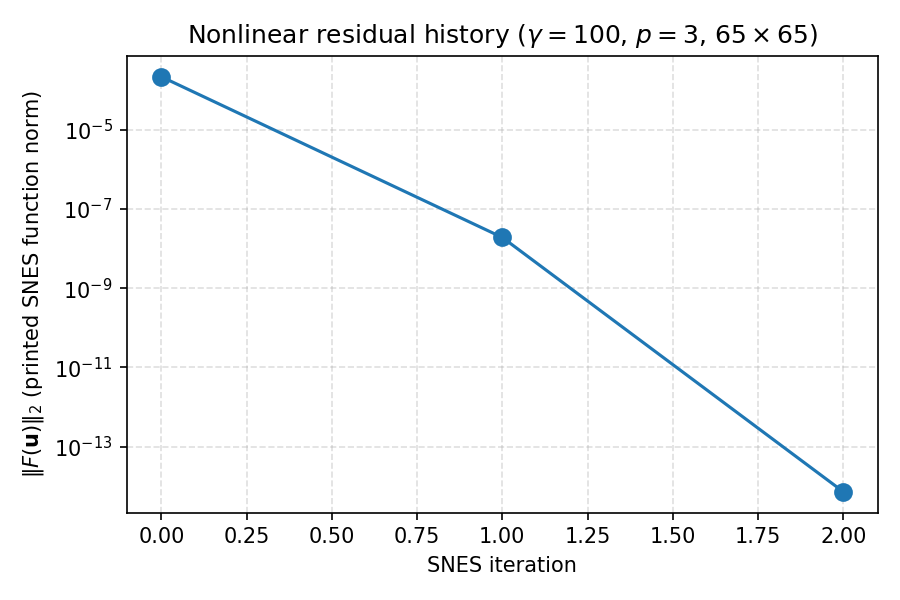
\includegraphics[width=0.65\linewidth]{snes_residual_history.png}
  \caption{Nonlinear residual $\|\mathbf{F}(\mathbf{u})\|_2$ vs.\ \texttt{SNES} iteration for $\gamma=100$, $p=3$, $65\times 65$.}
  \label{fig:snesres}
\end{figure}

\subsection*{Problem 7 --- \texttt{-rct\_linear\_f} and ParaView}

\paragraph{Run.}
\texttt{mpirun -n 1 ./reaction2d -rct\_p 3 -rct\_gamma 100 -rct\_linear\_f -da\_refine 3} (plus solver options as needed). This chooses $f=-\nabla^2 u_{\mathrm{exact}}$ while the PDE still contains $\gamma u^p$, so the Gaussian is \emph{not} an exact solution; the printed $\ell_2$ error vs.\ the same $u_{\mathrm{exact}}$ field is large ($\approx 0.41$ on $65\times 65$ in a sample run).

\paragraph{Visualization.}
Open the generated \texttt{reaction2d.vtr} in ParaView. Figure~\ref{fig:pv_linear_f} shows the computed field~\texttt{u} and, for comparison, the reference Gaussian $u_{\mathrm{exact}}$ stored in the same file (both on a $65\times 65$ grid, \texttt{-da\_refine~3}).

\begin{figure}[ht]
  \centering
  \begin{minipage}[t]{0.48\linewidth}
    \centering
    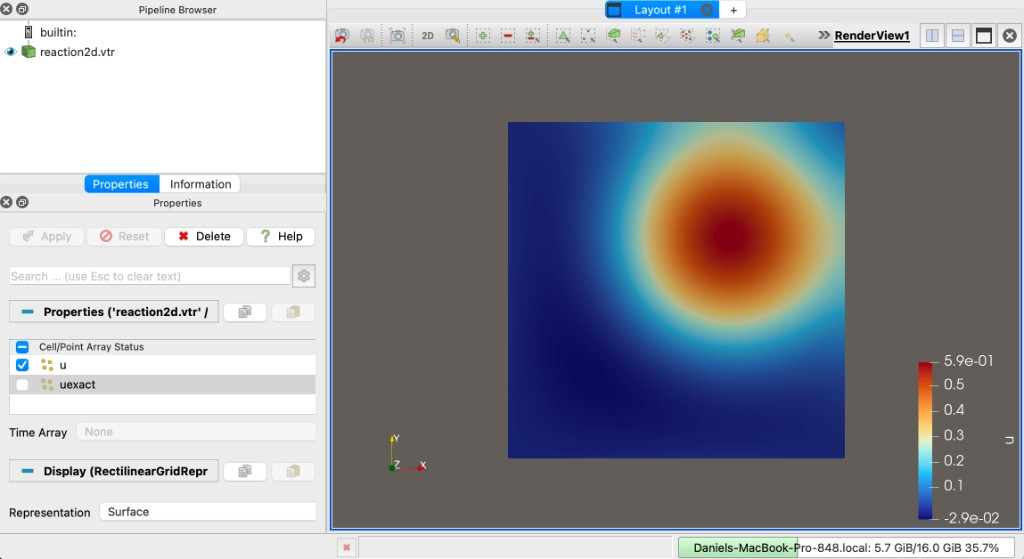
\includegraphics[width=\linewidth]{paraview_u.png}\\[0.4em]
    \small (a) Numerical solution $u$ with \texttt{-rct\_linear\_f}, $\gamma=100$, $p=3$.
  \end{minipage}
  \hfill
  \begin{minipage}[t]{0.48\linewidth}
    \centering
    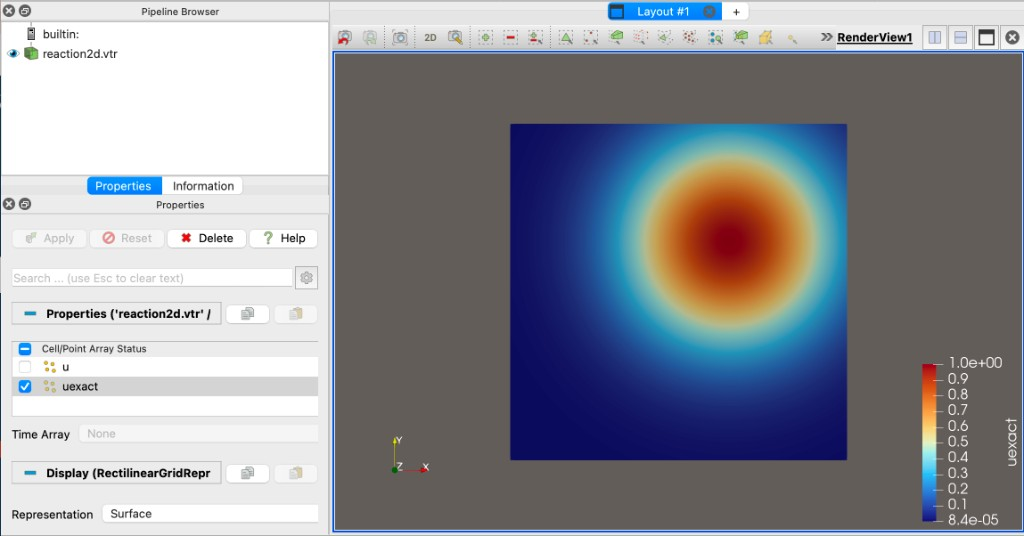
\includegraphics[width=\linewidth]{paraview_uexact.png}\\[0.4em]
    \small (b) Reference field $u_{\mathrm{exact}}$ (manufactured Gaussian).
  \end{minipage}
  \caption{ParaView screenshots for Problem~7: \texttt{reaction2d.vtr} colored by \texttt{u} and by \texttt{uexact}.}
  \label{fig:pv_linear_f}
\end{figure}

\paragraph{Discussion.}
For $\gamma=0$, the solution is diffuse/smooth at the MMS scale. With $\gamma>0$ the reaction term steepens and localizes the response where $u_{\mathrm{exact}}$ is large. With \texttt{-rct\_linear\_f} and $\gamma=100$, the forcing is ``linear Poisson'' but the equation retains $\gamma u^3$, so the solver balances an incompatible interior source with the boundary data; the field differs strongly from both the $\gamma=0$ case and from the Gaussian.

Visually, panel~(b) ($u_{\mathrm{exact}}$) shows a \emph{smoother} radial bump, but the \emph{outer} edge of the high-value region reads as more \emph{discrete}: on the fixed rectilinear grid, the steep decay of the Gaussian produces fairly sharp transitions between adjacent color bands, so the ``rim'' of the bump looks like a stepped contour rather than a perfectly smooth circle. Panel~(a) (numerical~$u$) is smoother in that transition region because the computed field is diffused and reshaped by the discrete Laplacian and the cubic nonlinearity; the mismatch between interior PDE and boundary data also flattens and shifts the response relative to the exact Gaussian.

\subsection*{Problem 8 --- Scaling ($-da\_refine=2,\ldots,6$; $1,2,4$ processes)}

\paragraph{Procedure.}
Nonlinear problem ($\gamma=100$, $p=3$) with the same direct linear solver as above; record wall time with \texttt{/usr/bin/time -p} or \texttt{-log\_view}. Raw numbers are archived in \path{homework3/solutions/logs/scaling_hw3_runs.txt}; the helper script is \path{homework3/solutions/run_scaling_study.sh}.

\begin{table}[ht]
  \centering
  \caption{Sample scaling (wall seconds from \texttt{time -p}; $\gamma=100$, $p=3$, \texttt{mumps}). Relative error is independent of $n_p$ (same discrete solution).}
  \begin{tabular}{r|r|r|r|r|r|r}
  \texttt{-da\_refine} & grid & $n_p=1$ & $n_p=2$ & $n_p=4$ & SNES & $\|\mathbf{e}\|_2/\|\mathbf{u}_{\mathrm{ex}}\|_2$ \\
  \hline
  2 & $33^2$   & 0.25 & 0.21 & 0.21 & 2 & $8.10\times 10^{-4}$ \\
  3 & $65^2$   & 0.19 & 0.19 & 0.22 & 2 & $2.03\times 10^{-4}$ \\
  4 & $129^2$  & 0.25 & 0.27 & 0.33 & 2 & $5.06\times 10^{-5}$ \\
  5 & $257^2$  & 0.52 & 0.50 & 0.51 & 2 & $1.27\times 10^{-5}$ \\
  6 & $513^2$  & 1.55 & 1.43 & 1.39 & 1 & $3.17\times 10^{-6}$ \\
  \end{tabular}
\end{table}

\paragraph{Visual summary.}
The next figure shows the same scaling experiment on log--log axes (base $9\times 9$ \texttt{DMDA} with \texttt{-da\_refine} $2,\ldots,6$, so $N=33,\ldots,513$). Wall times come from \texttt{/usr/bin/time -p} on a laptop; they are useful for trends but noisy at sub-second scale.

\begin{figure}[ht]
  \centering
  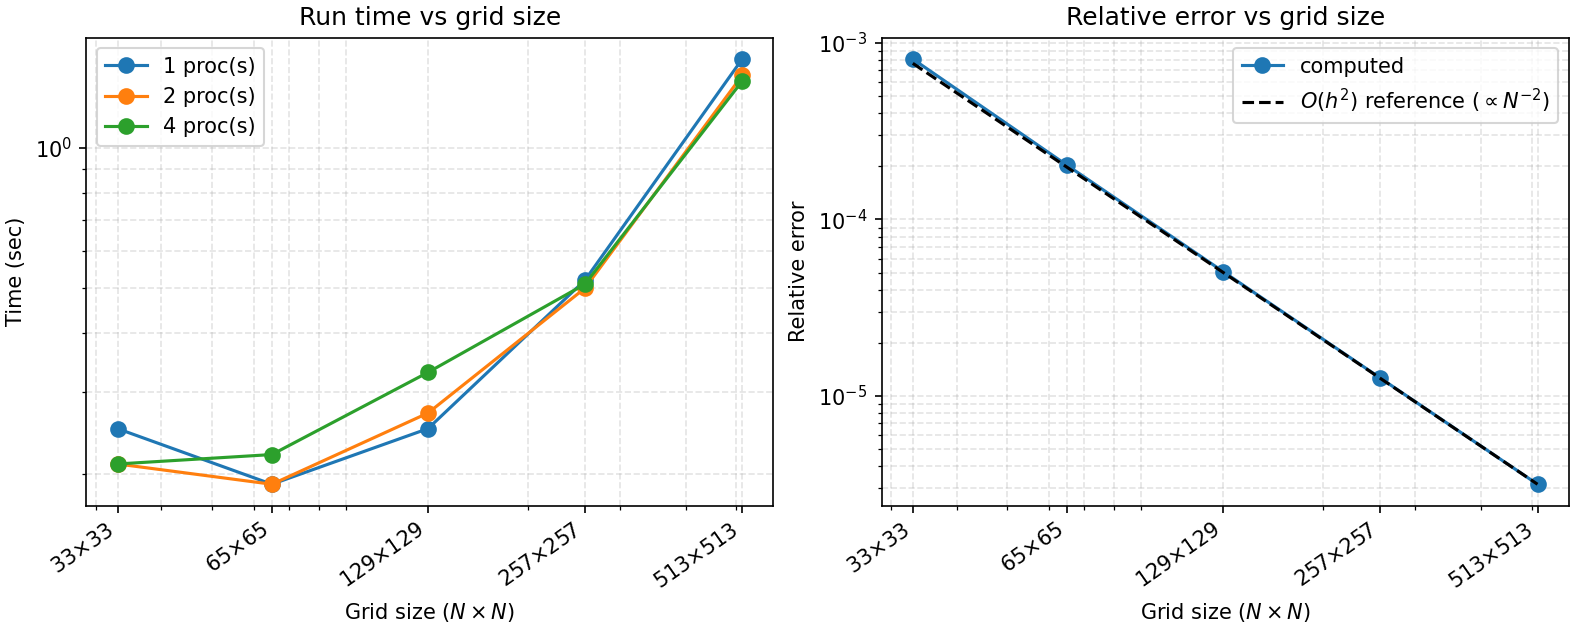
\includegraphics[width=\textwidth]{scaling_runtime_error.png}
  \caption{\textbf{Left:} wall-clock time vs.\ $N$ for $n_p\in\{1,2,4\}$ MPI processes. All curves rise with $N$ as the sparse-direct factorization and solve work grow; the three lines stay close because the problem is small and parallel overhead can offset gains. \textbf{Right:} relative error $\|\mathbf{u}-\mathbf{u}_{\mathrm{exact}}\|_2/\|\mathbf{u}_{\mathrm{exact}}\|_2$ vs.\ $N$ (any $n_p$; same discrete solution). The dashed curve is an $O(h^2)$ template $\propto N^{-2}$ fixed to match the finest-grid error---the measured points lie near it, consistent with a second-order stencil. Regenerate with \texttt{solutions/plot\_scaling\_figures.py}.}
  \label{fig:scaling_hw3}
\end{figure}

\paragraph{Interpretation.}
The left panel makes the \emph{weak-scaling} trend in problem size explicit: time increases superlinearly in this range as $N$ grows. The right panel isolates \emph{accuracy}: each refinement roughly quarters the error when $h$ is halved. The left panel is \emph{not} a clean strong-scaling speedup study---for that, $N$ should be large enough that parallel factorization dominates and/or an iterative preconditioned Krylov solver should replace full sparse LU.

\paragraph{Comments.}
\textbf{Problem size:} relative discretization error shrinks roughly by a factor of four when $h$ is halved, consistent with a second-order scheme (Fig.~\ref{fig:scaling_hw3}, right). \textbf{Strong scaling:} for these small test cases the LU factorization and sequential phases dominate, so increasing ranks does not reduce wall time much (sometimes slightly worse due to communication). A fair scaling study would use larger grids, iterative solvers with domain decomposition, and/or a cluster where direct solves are the bottleneck at scale.

  \end{document}